\section{Pulidos}
El pulido es un procedimiento que se realiza al momento de realizar empalmes en la fibra óptica, estos empalmes tienen que tener la menor cantidad de desperfectos para que su uso sea eficiente y no haya fallas ni perdidas durante su transmisión. Esto permite que los extremos de las fibras a empalmar sean complementarias y se pueda tener un empalme perfecto.
\subsection{Pérdida de Retorno}
La pérdida de retorno RL es una medida de la porción de luz que se refleja de regreso a la fuente en la unión. Usualmente medida en decibelios (\textit{dB.})
$$
RL(dB)= 10\cdot \log_{10} \Bigg(\dfrac{P_i}{P_r}\Bigg)
$$
\subsection{Tipos de Pulidos}
En los primeros días de los conectores de fibra óptica, las superficies frontales contiguas se pulían en un ángulo de $90^{\circ}$ con respecto al eje de la fibra, mientras que los estándares actuales requieren pulido por \textbf{PC} o pulido \textbf{APC}.

\subsubsection*{Flat Fiber Connector}
El conector de fibra original; es una conexión de superficie plana. El problema principal es que un pequeño espacio de aire entre las dos férulas\footnote{Esta es una estructura delgada (a menudo cilíndrica) que en realidad sostiene la fibra de vidrio.} se deja naturalmente cuando se acopla. Esto se debe en parte a que la cara extrema relativamente grande del conector permite que se acumulen numerosas imperfecciones leves pero significativas en la superficie.
\begin{center}
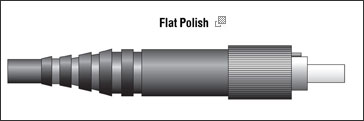
\includegraphics[scale=0.5]{flat}
\end{center}
\subsubsection*{Physical Contact (PC)}
Esta forma de pulido tiene un ligero diseño esférico para reducir el tamaño total de la cara final, lo que ayuda a disminuir el problema de espacio de aire que enfrentan los conectores de fibra plana. Resulta en una pérdida de retorno óptico más baja y se envía menos luz hacia la fuente de alimentación.
\begin{center}
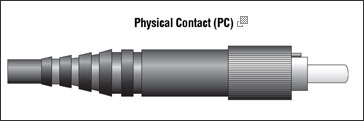
\includegraphics[scale=0.5]{pc}
\end{center}
\subsubsection*{Ultra-Physical Contact (UPC)}
Basándose en el PC, pero utilizando un método de pulido extendido se crea un acabado de superficie de fibra aún más fino. Tiene una reflexión posterior inferior que un conector de PC estándar y permite señales más confiables en TV digital, telefonía y sistemas de datos. El conector de fibra UPC podría usarse con fibra monomodo y fibra multimodo.
\begin{center}
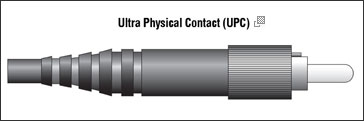
\includegraphics[scale=0.5]{upc}
\end{center}
\subsubsection*{Angled Physical Contact (APC)}
Es un tipo de pulido que esta cortado a un angulo de $8^{\circ}$ . Cuando se compara con un PC un APC muestra que tiene mejor reflectancia, porque su angulo pulido reduce la cantidad de luz reflejada a la interfaz de conector.
\begin{center}
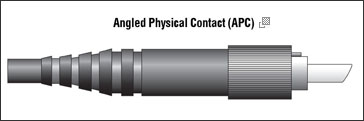
\includegraphics[scale=0.5]{apc}
\end{center}
\section{Conectores}
Los conectores de fibra óptica son únicos. Los cables de fibra transmiten pulsos de luz en lugar de señales eléctricas, por lo que las terminaciones deben ser mucho más precisas. En lugar de simplemente permitir que los pines hagan contacto metal con metal, los conectores de fibra óptica deben alinear perfectamente las fibras de vidrio para permitir la comunicación. Si bien hay muchos tipos diferentes de conectores de fibra, comparten características de diseño similares.
\subsubsection*{Standard Connector (SC)}
El SC fue creado a mediados de los 80 por la empresa de telecomunicaciones Nippon Telegraph and Telephone, y fue uno de los primeros conectores en llegar al mercado tras la llegada de las férulas de cerámica. A veces se lo denomina "conector cuadrado".
\begin{center}
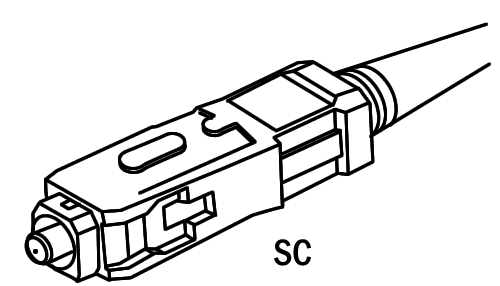
\includegraphics[scale=0.75]{SC_CON}
\end{center}
\subsubsection*{Lucent Connector (LC)}
El LC, también conocido como Little Connector, fue creado por Lucent Technologies es extensamente utilizado en aplicaciones mono modo ya que tiene un excelente rendimiento y puede ser terminado de manera sencilla. Considerado por algunos como el reemplazo moderno del conector SC, la introducción del conector LC tuvo menos éxito, en parte debido a las altas tarifas de licencia iniciales del inventor Lucent Corporation.
\begin{center}
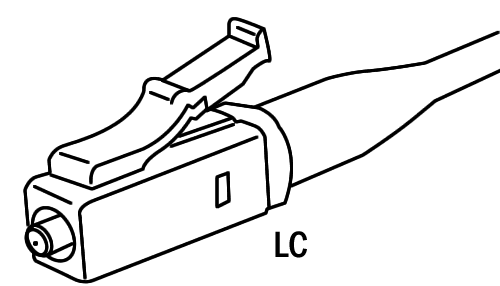
\includegraphics[scale=0.75]{LC_CON}
\end{center}
\subsubsection*{Straight Tip (ST)}
El conector ST fue uno de los primeros tipos de conector ampliamente implementado en aplicaciones de redes de fibra óptica. Desarrollado originalmente por AT\& T.
\begin{center}
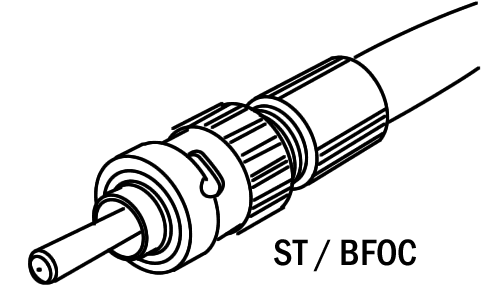
\includegraphics[scale=0.75]{ST_CON}
\end{center}
\subsubsection*{Ferrule Connector (FC)}
El conector de fibra FC fue el primer conector de fibra óptica que utilizó una férula de cerámica, pero a diferencia del conector SC y LC con cuerpo de plástico, utiliza un accesorio de tipo tornillo redondo hecho de acero niquelado o inoxidable. La cara del extremo del conector FC se basa en una clave de alineación para una inserción correcta y luego se aprieta en el adaptador / conector mediante un collar roscado.
\begin{center}
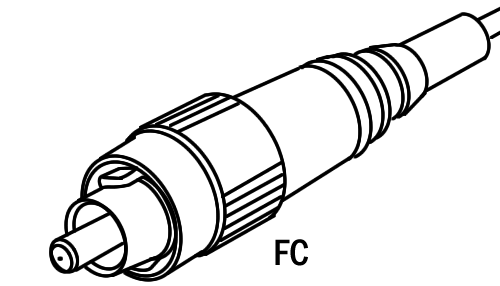
\includegraphics[scale=0.75]{FC_CON}
\end{center}
\subsubsection*{Mechanical Transfer-Registered Jack (MTRJ)}
Un conector de cable de fibra óptica que es muy popular para dispositivos de factor de forma pequeño debido a su pequeño tamaño. Al alojar dos fibras y acoplarse junto con los pines de ubicación en el enchufe, el MT-RJ proviene del conector MT, que puede contener hasta 12 fibras. Se utilizan para proporcionar velocidades de fibra óptica a computadoras personales, servidores, estaciones de trabajo comerciales, enrutadores inalámbricos, módems y otros dispositivos que aún no han sido equipados para su uso con cables de fibra óptica. Los conectores MTRJ son, por lo tanto, un tipo de conector híbrido entre un cable de fibra óptica y un cable Ethernet.

\begin{center}
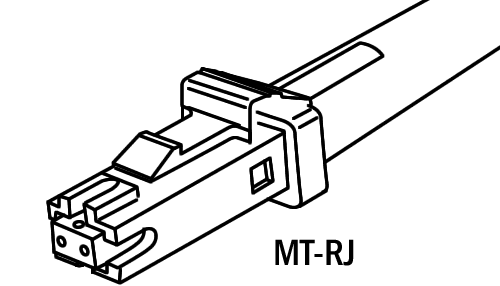
\includegraphics[scale=0.75]{MTRJ_CON}
\end{center}
\subsubsection*{Multi-fiber Push-on (MTP/MPO)}
El conector de fibra MPO/MTP es un conector de fibra múltiple que combina fibras de 12 a 24 fibras en una única férula rectangular.
\begin{center}
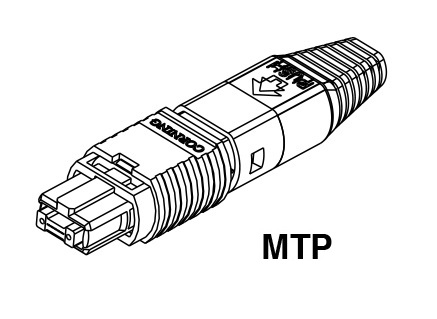
\includegraphics[scale=0.25]{MTP_CON}
\end{center}
\subsubsection*{Diferencias MTP \& MPO}
El MPO (Multiple-Fiber Push-on/Pull-off) se utiliza en las aplicaciones de multifibra necesarias para la transmisión de alta velocidad de 40/100G y de mucha más velocidad. El MTP, por otro lado, es una marca registrada que cumple con el estándar MPO. Estos dos conceptos se utilizan indistintamente.

\section{Multiplexación por División de Longitud de Onda (Wavelength Division Multiplexing)}
Wavelength Division Multiplexing (WDM) es un avance importante en el historial de desarrollo de la tecnología de comunicación de fibra óptica. El principio básico del WDM es que las señales de luz con diferentes longitudes de onda se unen primero y luego se acoplan a líneas de cable de fibra óptica en las mismas fibras para la transmisión. Finalmente, el receptor separa las diferentes longitudes de onda mediante el procesamiento de la señal, restaura la señal original y las envía a diferentes terminales.
\begin{center}
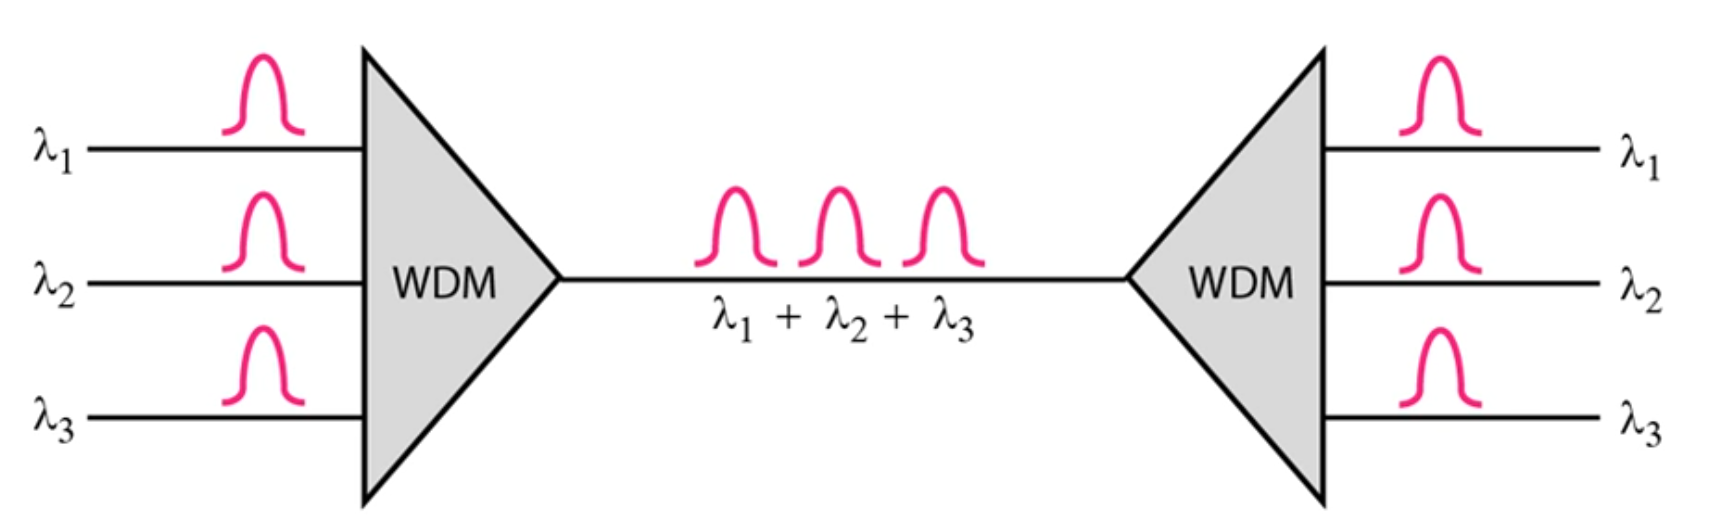
\includegraphics[scale=0.4]{WDM}
\end{center}
\subsection{Coarse WDM (CWDM)}
La multiplexación por división de longitud de onda gruesa (CWDM) es un método de combinación de múltiples señales en rayos láser en varias longitudes de onda para la transmisión a lo largo de cables de fibra óptica, de modo que el número de canales es menor que en la multiplexación por división de longitud de onda densa (DWDM) pero más que en la longitud de onda estándar división multiplexación (WDM).
\begin{center}
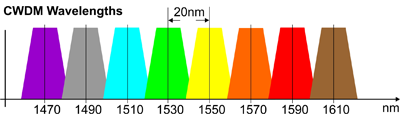
\includegraphics[scale=1.6]{CWDM}
\end{center}
\subsection{Dense WDM (DWDM)}
La multiplexación por división de longitud de onda densa (DWDM) es una tecnología que reúne (multiplexa) señales de datos de diferentes fuentes para que puedan compartir un solo par de fibra óptica mientras mantienen una separación completa de los flujos de datos. Cada señal se transporta en una longitud de onda de luz separada; La parte de \textit{densa} de DWDM se refiere al hecho de que más de 80 longitudes de onda separadas, cada una de aproximadamente 0.8 de un nanómetro (nm) de ancho, pueden compartir una sola fibra óptica.

\begin{center}
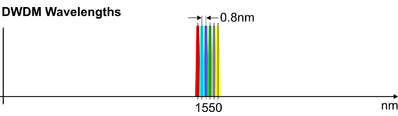
\includegraphics[scale=1.6]{DWDM}
\end{center}
% https://www.fibraopticahoy.com/tipos-conectores-fibra-optica/
% https://www.thefoa.org/Lennie/term.html
% https://lightbrigade.com/productionFiles/Resource-PDF/Whitepapers/Introduction-to-Connectors-Whitepaper-The-Light-Br.aspx
% http://www.fiberdk.dk/userfiles/pdf/b57563567a56066fa8d6d01d5f7580b9.pdf
% https://www.rp-photonics.com/passive_fiber_optics5.html
% https://www.ppc-online.com/blog/picking-the-right-fiber-connector-pc-upc-or-apc
% https://www.tonercable.com/pdf/Fiber_Optic_Tips_-_APC_vs_UPC.pdf
% http://www.fiber-optic-solutions.com/evolution-of-flat-pc-upc-and-apc-fiber-connectors.html
% https://www.newport.com/medias/sys_master/images/images/h3e/h84/8797095985182/Fiber-Preparation-Fiber-Connectors.pdf
% https://www.scte.org/TechnicalColumns/05-10-01%20return%20loss.pdf
% http://www2.optics.rochester.edu/users/gpa/opt428.htm
% https://www.rojone.com/assets/files/L-Com-15-Fiber-Optic.pdf
% https://store.cablesplususa.com/fiber-optic-connector-polish-information.html


% https://www.fs.com/mx/mtp-connector-vs-mpo-connector-what-is-the-difference-aid-936.html